% =====================================================================
%  Preprint draft, Springer LNCS format (MICCAI style).
%  Compile with pdfLaTeX + BibTeX (Overleaf default).
%  llncs.cls and splncs04.bst are included for convenience; Overleaf
%  also provides them.
%
%  TODO before posting:
%   - add Prof. Fady's surname and the exact department names below;
%   - every author reads every line and checks every number against
%     the repository (results/*.md);
%   - keep the "Use of AI tools" section.
% =====================================================================
\documentclass[runningheads]{llncs}

\usepackage[T1]{fontenc}
\usepackage{graphicx}
\usepackage{booktabs}
\usepackage{amsmath}
\usepackage{xcolor}
\usepackage{tikz}
\usetikzlibrary{positioning,arrows.meta,calc}
\usepackage{hyperref}
\usepackage{color}
\renewcommand\UrlFont{\color{blue}\rmfamily}
\urlstyle{rm}
\graphicspath{{figures/}}

\newcommand{\Astra}{GPT-6 Astra}

\begin{document}

\title{Can an LLM Write a Medical Classifier's Weights?\\
A Controlled Test of Weight-Space Programming on Pediatric Chest X-rays}

\titlerunning{Can an LLM Write a Medical Classifier's Weights?}

\author{Mahd Hindi\inst{1} \and
Khaled AlHassani\inst{1} \and
Abdullah AlKaabi\inst{1} \and
Fady~[SURNAME]\inst{1}}

\authorrunning{M. Hindi et al.}

\institute{College of Information Technology [check], United Arab Emirates University, Al Ain, United Arab Emirates\\
\email{mahmoud.alhindi@gmail.com}}

\maketitle

\begin{abstract}
Medical image classifiers are normally trained by gradient descent on labelled data.
A recent report claims that a frontier large language model (LLM) can instead write a network's weights directly.
But its successes came from tasks whose rules the model can read, such as game source code.
Whether this works on medical images, which have no written rules, and how it compares with fair baselines, is unknown.
We test it on pneumonia detection in pediatric chest X-rays, with patient-grouped splits and a held-out test collection.
An LLM wrote all weights of a small CNN under five information conditions.
We compared it with a random search given the same evaluation budget, and with gradient training of the same network.
Example images and practice scores alone were not enough.
With a report on its own network's channels, the LLM beat every matched random search and reached a test AUROC of 0.859, close to gradient training (0.882).
Editing the last layer of a fine-tuned ResNet-50 with the same kind of report raised its AUROC from 0.954 to 0.976, though re-training still did better.
A size-matched check shows that LLM-selected features rely more on an image-size shortcut than trained weights do.
LLM weight-writing works, but only with feedback on the network's internals.
\keywords{Large language models \and Weight-space programming \and Chest X-ray \and Shortcut learning \and Evaluation}
\end{abstract}

% =====================================================================
\section{Introduction}
Every weight of a deployed medical classifier is normally set by an optimiser that reads labelled data.
Takehi et al.~\cite{takehi2026} recently reported a different route, \emph{weight-space programming}: a general-purpose LLM, \Astra, reads a network's raw weights, reasons about what each part computes, and writes new values directly.
In their experiments it named the game a policy network plays from its weights alone, repaired a stalled driving policy by editing 3.5\,\% of its weights, removed a repetition loop from a small language model, and wrote game-playing networks from an all-zero start that beat a PPO agent trained for 100 million steps.

Two features of that work limit what it says about medicine.
First, the successes came either from tasks whose rules the LLM can read (game source code, a simulator) or from models with one clear fault to remove; a medical image has neither a specification nor a single bug.
Second, the report is an early, non-peer-reviewed blog post, and medical tasks were outside its scope.
LLM-driven program search has produced verified results in mathematics~\cite{romeraparedes2024}, and networks that generate other networks' weights have a long history~\cite{ha2017}, but we know of no controlled test of an LLM writing a medical classifier's weights.

We provide one on the Kermany pediatric chest X-ray dataset~\cite{kermany2018}, a benchmark on which image-level splits inflate reported accuracy~\cite{singh2024}, so we keep patients separate and score once on the official test collection.
Our question is: \emph{can an LLM, writing every weight by reasoning, beat a random search given the same number of practice evaluations, and how close does it come to gradient training of the same network?}

\noindent\textbf{Main contributions.}
\begin{enumerate}
\item The first controlled test of LLM weight-space programming on a medical imaging task, in three modes: writing a CNN from scratch, writing the final layer of a frozen pretrained network, and editing a fine-tuned network.
\item A fair protocol: patient-grouped splits, a held-out test collection scored once, a random search matched to the LLM's evaluation budget, a mechanical selection rule, and gradient training of the identical architecture.
\item An ablation over what the LLM is given, showing that example images add little, practice scores help, and a report on the network's own channels is what brings it close to training; a second LLM reproduces the result.
\item A size-matched robustness check showing that the features an LLM selects from such reports rely more on an acquisition-size shortcut~\cite{zech2018,geirhos2020,degrave2021} than trained weights do.
\end{enumerate}

% =====================================================================
\section{Method}

\begin{figure}[t]
\centering
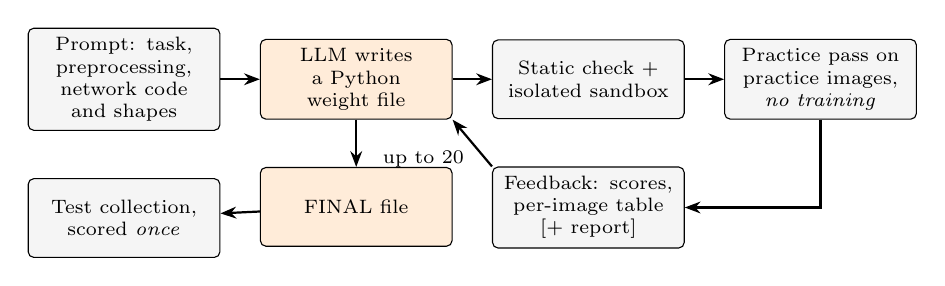
\begin{tikzpicture}[
  node distance=5mm and 5mm,
  box/.style={draw, rounded corners=2pt, align=center, font=\scriptsize, minimum height=10mm, text width=22mm, fill=gray!8},
  hot/.style={box, fill=orange!15},
  arr/.style={-{Stealth[length=2mm]}, thick}]
\node[box] (prompt) {Prompt: task, preprocessing, network code and shapes};
\node[hot, right=of prompt] (llm) {LLM writes a Python weight file};
\node[box, right=of llm] (check) {Static check +\\ isolated sandbox};
\node[box, right=of check] (pass) {Practice pass on practice images, \emph{no training}};
\node[box, below=6mm of check] (fb) {Feedback: scores, per-image table [+ report]};
\node[hot, below=6mm of llm] (final) {FINAL file};
\node[box, below=6mm of prompt] (test) {Test collection, scored \emph{once}};
\draw[arr] (prompt) -- (llm);
\draw[arr] (llm) -- (check);
\draw[arr] (check) -- (pass);
\draw[arr] (pass.south) |- (fb.east);
\draw[arr] (fb.north west) -- node[below left=-1pt, font=\scriptsize, align=right] {up to 20} (llm.south east);
\draw[arr] (llm) -- (final);
\draw[arr] (final) -- (test);
\end{tikzpicture}
\caption{The practice loop. Each condition is a fresh LLM chat. The LLM returns a file that builds every weight; a static check and a sandbox enforce the rules before the weights are loaded. Practice passes return feedback on practice images only; the LLM decides when to stop, and its FINAL file is scored once on the test collection. Conditions differ only in what the prompt and the feedback contain (Table~\ref{tab:conds}).}
\label{fig:loop}
\end{figure}

\subsection{Networks the LLM writes}
\noindent\textbf{Small CNN.}
\texttt{WrittenCNN} has conv1 ($1\!\to\!16$, $5\times5$, stride~2), ReLU and $2\times2$ max-pooling, conv2 ($16\!\to\!32$, $3\times3$), ReLU and max-pooling, a $4\times4$ adaptive average pool, and one linear unit ($512\!\to\!1$): 5,569 parameters.
The same architecture is used by the LLM, by the random rivals and by gradient training, so model size is identical across compared rows.

\noindent\textbf{Final layer of a frozen pretrained network.}
For condition G the backbone is an ImageNet ResNet-50~\cite{he2016} (\texttt{IMAGENET1K\_V2}), never trained on X-rays and kept frozen; the LLM writes only the final layer (2,048 weights and a bias), starting from zeros.

\noindent\textbf{Editing a fine-tuned network.}
For conditions E and H the network is our own ResNet-50, fully fine-tuned on the training split; the LLM receives its current final layer and edits it.

\subsection{Information conditions}
Table~\ref{tab:conds} lists what each condition gives the LLM.
Every condition receives the exact architecture, the preprocessing code path and the scoring rule, but not the dataset's name or class proportions.
In a \emph{practice pass} the LLM sends a complete weight file, which we run once, with no training, on the next 256 of 782 practice images (cycling), returning AUROC, accuracy, sensitivity, specificity, per-class mean probability and a per-image score table.
The \emph{channel report} (F) adds, for each of the 16 conv1 and 32 conv2 channels, the mean activation per class, its \emph{separation} (the AUROC of that channel's mean activation alone), the share of images on which it is silent, and, for conv2, its mean contribution to the logit per class.
The \emph{feature report} (G, H) gives the same statistics for each of the 2,048 ResNet-50 features, sorted by separation; no images are attached in G, E or H because those features have no names.
F was run in three independent chats; every other condition in one.

\begin{table}[t]
\centering
\caption{Information conditions. Letters follow the order in which conditions were run; rows are ordered by how much information the LLM receives.}
\label{tab:conds}
\setlength{\tabcolsep}{2.5pt}
\scriptsize
\begin{tabular}{@{}llccl@{}}
\toprule
 & Network and task & Examples & Practice passes & Feedback \\
\midrule
A & Small CNN, write all weights & -- & -- & -- \\
C & Small CNN, write all weights & 16 & -- & -- \\
B & Small CNN, write all weights & -- & up to 20 & scores only \\
D & Small CNN, write all weights & 16 & up to 20 & scores only \\
F & Small CNN, write all weights & 16 & up to 20 & + channel report \\
\midrule
G & Frozen ImageNet ResNet-50, write last layer & -- & up to 20 & + feature report \\
E & Fine-tuned ResNet-50, edit last layer & -- & up to 20 & scores only \\
H & Fine-tuned ResNet-50, edit last layer & -- & up to 20 & + feature report \\
\bottomrule
\end{tabular}
\end{table}

\subsection{Rules}
The LLM returns a Python file that builds each array from constants and formulas, importing only \texttt{numpy} and \texttt{math}; it may not read files, call the network or draw random numbers.
A static check and an isolated subprocess enforce these restrictions before any weight is loaded.
The prompts forbid optimisation, gradient estimation, finite differences, search loops, and any weight computed as a formula of the reported numbers (for example, setting a weight proportional to a channel's separation).
Every change must be designed and explained; the transcripts were checked against these rules before the FINAL file was scored.

\subsection{Rivals}
\noindent\textbf{Matched random search}~\cite{bergstra2012}.
We draw $N$ random networks (PyTorch default initialisation), score each on the same $N$ practice slices the LLM saw, and keep the best; $N$ is the number of practice evaluations the matching LLM run used (10 for B, 11 for D and for the second LLM, 4--5 for the F runs, 17 for G).
Each search is repeated 100 times.
A \emph{random-initialisation floor} scores 200 untrained networks with no selection.

\noindent\textbf{Selection rule} (G only).
The mechanical version of ``read the report and keep what separates'': keep the top-$k$ features by $|\text{separation}-0.5|$ on the practice images, with weights $\pm1/(k\sigma)$ and $k\in\{8,32,128,512\}$ chosen on those images; no gradients.

\noindent\textbf{Gradient training.}
The same small CNN trained with AdamW (learning rate $10^{-3}$, 12 epochs, checkpoint by validation AUROC, seeds 42 and 43); for G, a logistic-regression linear probe on the frozen features of the 4,424 training images ($C$ chosen on the practice set); for E and H, the threshold moved by Youden's index on the practice images, and the final layer re-trained by logistic regression on the same practice images.

% =====================================================================
\section{Experimental Setup}

\noindent\textbf{Dataset.}
The Kermany pediatric chest X-ray collection~\cite{kermany2018} contains frontal radiographs of children aged one to five labelled normal or pneumonia.
Images are converted to 8-bit grayscale, padded to a square with black bars and resized to $224\times224$.
After byte-identical duplicates are removed, the training pool is split \emph{by patient} (seed 42) into 4,424 training and 782 validation images; the validation images serve as the \emph{practice set}, the only source of LLM feedback for A--G.
The official test folder (618 images: 231 normal, 387 pneumonia) is a separately collected set and is scored once per condition.
No child appears in two splits.
Because the fine-tuned ResNet-50 is already near-perfect on the practice set (AUROC 0.9995), E and H take practice feedback from one patient-grouped half of the test folder (306 images) and are scored on the other half (312 different children).

\noindent\textbf{Size-matched subset.}
On the test folder, the original image height alone separates the classes (AUROC 0.921), because pneumonia files are smaller.
We pair each normal test image greedily (random order, seed 0) with an unused pneumonia image whose original width and height are both within about 5\,\%, giving 70 pairs (140 images).
On this subset height alone scores 0.510 and aspect ratio 0.500; a model that ranks by size should fall toward 0.5.

\noindent\textbf{Implementation details.}
The LLMs were \Astra{} and, for one F chat, Claude Fable 5.2 (Anthropic), each used through its chat interface with no tools except, in G, plain file reads of the long reports.
Each chat was started fresh, from an empty project folder, so that no earlier condition was visible.
All network evaluation and training ran on one NVIDIA T4 GPU (Google Colab).
Training the small CNN takes 3.3\,min per seed; an LLM run on the small CNN took 20--72\,min of wall-clock time from the first to the last practice pass, including manual copy-paste.
The primary metric is test AUROC with a 95\,\% bootstrap confidence interval (1,000 resamples); accuracy, sensitivity and specificity are reported at $P{=}0.5$.
All prompts, transcripts, weight files, practice logs and result files are public~\cite{repo}.

% =====================================================================
\section{Results}

\begin{table}[t]
\centering
\caption{Small CNN (5,569 parameters) on the official test folder ($n{=}618$). Brackets: 95\,\% bootstrap CI for single runs; 5th--95th percentile for random rows. $\pm$: SD over chats or seeds.}
\label{tab:main}
\setlength{\tabcolsep}{3pt}
\scriptsize
\begin{tabular}{@{}lcccc@{}}
\toprule
Weights obtained by & Test AUROC & Sens. & Spec. & Evaluations \\
\midrule
A\; LLM, zero-shot & 0.519 [0.473, 0.565] & 0.74 & 0.23 & 0 \\
C\; LLM, 16 example images & 0.599 [0.553, 0.646] & 0.89 & 0.14 & 0 \\
B\; LLM, practice scores & 0.737 [0.695, 0.779] & 0.59 & 0.82 & 10 \\
D\; LLM, images + practice scores & 0.745 [0.705, 0.785] & 0.69 & 0.72 & 11 \\
\textbf{F\; LLM, + channel report} (3 chats) & \textbf{0.859\,$\pm$\,0.016} & 0.91 & 0.50 & 4--5 \\
\quad runs 1 / 2 / 3 & 0.876 / 0.865 / 0.838 & & & \\
F\; second LLM (Claude Fable 5.2), 1 chat & 0.876 [0.850, 0.904] & 0.88 & 0.73 & 11 \\
\midrule
Random initialisation, no selection (200) & 0.491 [0.245, 0.752] & -- & -- & -- \\
Best of 4 random networks (100 searches) & 0.691 [0.432, 0.769] & -- & -- & 4 \\
Best of 10 random networks (100 searches) & 0.716 [0.573, 0.786] & -- & -- & 10 \\
Best of 11 random networks (100 searches) & 0.719 [0.632, 0.790] & -- & -- & 11 \\
Gradient training, same CNN (2 seeds) & 0.882\,$\pm$\,0.012 & 0.97 & 0.49 & -- \\
\midrule
\emph{Reference:} fine-tuned ResNet-50 (23.5\,M params) & 0.971\,$\pm$\,0.001 & 1.00 & 0.64 & -- \\
\bottomrule
\end{tabular}
\end{table}

\subsection{Writing a CNN from scratch}
Table~\ref{tab:main} gives the main comparison.
Every F chat beat every matched random search: over 100 repetitions, the best-of-4 and best-of-5 searches never exceeded 0.821.
The three chats averaged 0.859\,$\pm$\,0.016, 0.023 below gradient training of the same network (0.882\,$\pm$\,0.012), with overlapping confidence intervals.
Both trail the fine-tuned ResNet-50 by about 0.1.
Like the trained networks, the LLM-written networks have high sensitivity and low specificity at $P{=}0.5$ on this test collection, a calibration problem rather than a ranking one.

\begin{figure}[t]
\centering
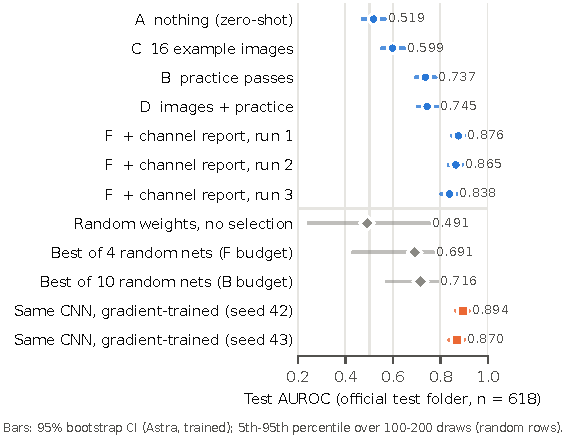
\includegraphics[width=0.82\textwidth]{project_ladder.pdf}
\caption{Ablation over what the LLM receives (test AUROC, $n{=}618$). Example images add 0.08 (C vs.\ A); practice scores add 0.22 (B vs.\ A); images on top of practice add 0.01 (D vs.\ B); the channel report adds a further 0.11 (F vs.\ D). Every F run lies above the 95th percentile of its matched random search.}
\label{fig:ladder}
\end{figure}

\noindent\textbf{Ablation: what the LLM needs.}
Fig.~\ref{fig:ladder} separates the contributions.
With no feedback the LLM is at chance, and looking at 16 example images helps little.
Practice scores are what make it work, but B (0.737) is not clearly better than its matched random search: 28\,\% of best-of-10 searches score as high.
Adding the images on top of practice changes almost nothing (D, 0.745).
The channel report adds a further 0.11 after only four or five evaluations, more than the scores-only conditions gained in ten or eleven.

\noindent\textbf{What the LLM wrote.}
The three F chats began from different first designs (brightness, opacity and texture mixtures, 0.59--0.63 practice AUROC).
In each, after the first channel report, the LLM noticed that its own \emph{texture} channels (edge magnitude or local intensity range) were consistently higher on normal images, and rebuilt the readout around them with round-number negative weights; practice AUROC rose to 0.89--0.93 in the next pass.
Run 3's final network reads a single channel (mean edge magnitude, weight $-1$ per grid cell, bias $+1.25$).
The report therefore acts as a label-informed \emph{feature-selection} signal: the LLM designs a filter bank from domain knowledge, and the report tells it which of its own filters separate the classes.
This is reasoning rather than training, but it is not data-free.
The random search also selects on practice labels, but over whole networks, and its winners overfit the practice slices (median practice AUROC 0.84, test 0.69), whereas the F networks keep a smaller gap (practice 0.93, test 0.86).

\noindent\textbf{A second LLM.}
One F chat with Claude Fable 5.2, using the identical prompt, reached 0.876 [0.850, 0.904], equal to the best Astra run, with better balance (specificity 0.73 vs.\ 0.40), after 11 evaluations; no best-of-11 random search reached it (maximum 0.854).
It converged on the same rule (capped edge energy in the central lung cells), added zero-weight ``probe'' channels to measure per-cell class differences, and excluded the padded image borders after judging from the example images that padding was an acquisition artefact.

\begin{table}[t]
\centering
\caption{Final layers on frozen and fine-tuned ResNet-50 features. G is scored on the full test folder ($n{=}618$; size-matched subset 140 images). E and H are scored on the 312-image scoring half (size-matched pairs within it: 72 images).}
\label{tab:resnet}
\setlength{\tabcolsep}{3pt}
\scriptsize
\begin{tabular}{@{}lcccc@{}}
\toprule
Final layer obtained by & Test AUROC & Spec. & Features & Size-matched \\
\midrule
\multicolumn{5}{@{}l}{\emph{G: frozen ImageNet ResNet-50, layer written from zeros} ($n{=}618$)} \\
\textbf{LLM, 17 passes + feature report} & \textbf{0.902} [0.877, 0.922] & 0.59 & 26 & 0.724 \\
Selection rule (no LLM, no gradients) & 0.883 [0.853, 0.905] & 0.80 & 32 & 0.669 \\
Best of 17 random layers (median of 100) & 0.678 [0.573, 0.781] & -- & 2,048 & 0.571 \\
Linear probe, trained & 0.947 [0.926, 0.963] & 0.53 & 2,047 & 0.862 \\
\midrule
\multicolumn{5}{@{}l}{\emph{E, H: fine-tuned ResNet-50, layer edited} ($n{=}312$)} \\
Unedited & 0.954 [0.925, 0.977] & 0.50 & 2,048 & 0.879 \\
Threshold moved (Youden on practice half) & 0.954 [0.925, 0.977] & 0.89 & 2,048 & 0.879 \\
E\; LLM edit, scores only & 0.954 [0.925, 0.977] & 0.64 & 2,048 & -- \\
\textbf{H\; LLM edit, + feature report} & \textbf{0.976} [0.959, 0.990] & 0.83 & 49 & 0.922 \\
Re-trained on the same 306 practice images & 0.985 [0.974, 0.995] & 0.91 & 2,048 & 0.925 \\
\bottomrule
\end{tabular}
\end{table}

\subsection{Pretrained features: writing and editing a final layer}
\noindent\textbf{G: writing a layer on frozen features.}
The LLM used 17 of its 20 passes, changing one thing at a time, and wrote a layer with 26 hand-picked features (weights $+4$, $-2$, $\pm1$, $\pm0.5$, $-0.25$; bias 0).
It reached 0.902, above the small-CNN result and far above random search (maximum 0.800); the mechanical selection rule scored 0.883, with overlapping intervals (Table~\ref{tab:resnet}).
The trained probe reached 0.947, a gap of 0.045, twice the gap on the small CNN: with 2,048 unnamed features the LLM can only shortlist a few dozen that separate on practice images, whereas training uses them jointly.
The LLM forecast about 0.96 and warned that 17 looks at the practice set made its practice scores (0.96--0.98) optimistic.

\noindent\textbf{E, H: editing a fine-tuned network.}
With scores only (E), the LLM could only move the operating point: AUROC stayed at 0.954, and simply moving the threshold gave better balanced accuracy (0.914 vs.\ 0.814).
With the feature report (H), it changed the ranking: after three adjustments it replaced the trained layer with $\pm1$ votes on 49 features plus a bias of $-2$, and AUROC rose to 0.976.
Re-training the layer by logistic regression on the same 306 practice images still did better (0.985).
On all 618 test images the unedited model scores 0.966; the scoring half is harder.

\begin{figure}[t]
\centering
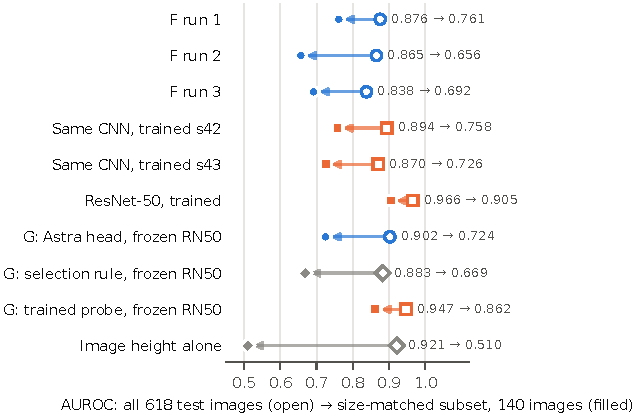
\includegraphics[width=0.86\textwidth]{project_robust.pdf}
\caption{Size-matched check. Open markers: all 618 test images; filled: 140 images matched for original width and height. Image height alone drops to chance, so the check removes the shortcut. Every model loses AUROC, but LLM-written networks and LLM-selected features lose more than trained weights on the same input.}
\label{fig:robust}
\end{figure}

\subsection{Shortcut check: part of every score is image size}
Fig.~\ref{fig:robust} shows that every model loses AUROC on the size-matched subset, so part of every score on this collection comes from acquisition size.
The F networks fall from 0.859 to 0.703 on average (0.761, 0.656, 0.692; every 95\,\% CI stays above 0.5), the same CNN trained by gradient descent from 0.882 to 0.742, and the fine-tuned ResNet-50 from 0.966 to 0.905.
On frozen features the gap is larger: the trained probe keeps 0.862, whereas the LLM's 26 features fall to 0.724 and the selection rule to 0.669.
The mechanism is visible in the data: pneumonia files are smaller, so after resizing they show less fine texture, and a ``less texture means pneumonia'' rule reads both the disease (consolidation smooths the lung pattern) and the file size.
Within each class, F2 and F3 scores correlate with log image height (Spearman $\rho$ from $-0.48$ to $-0.72$), as do the trained CNN's ($-0.59$ to $-0.74$).
Features chosen because they separate the practice images best tend to be the ones that also track size, whereas a probe spreading weight over all 2,048 features is less exposed.
In every F chat the LLM itself warned that the texture cue might reflect acquisition or processing rather than disease.
On the fine-tuned network the LLM's edit is not more size-dependent than re-training (0.922 vs.\ 0.925): fine-tuned features already track the disease.
This matches shortcut learning reported for chest X-ray models~\cite{zech2018,degrave2021}, and it means that a report-driven LLM can find a shortcut as readily as a signal.

% =====================================================================
\section{Discussion and Conclusion}
On a medical task with no written rules, an LLM can write a working classifier's weights, but only with feedback about the internals of its own network.
With that feedback it beats a random search given the same budget in every chat, comes within 0.023 AUROC of gradient training on a small CNN, and improves a fine-tuned ResNet-50 from 0.954 to 0.976.
Gradient training on the same information still wins in every comparison (0.882, 0.947, 0.985), and the features the LLM selects lean more on an acquisition shortcut.
The value of the approach is therefore not accuracy but legibility: every weight comes with a stated reason, and the LLM flagged the shortcut it was exploiting.

\noindent\textbf{Limitations.}
We used one dataset from one hospital; the size-matched subset is small (140 images) and atypical, so its absolute AUROC values matter less than the comparison between models.
F has three chats and every other condition one; the second LLM ran one F chat and was not put through the size-matched check.
The loop was run by hand, which caused one log reset (F run 1, after which the matched rival was set to the evaluations actually used); a separate re-run is documented in the repository and gave the LLM no extra information.
E and H take practice feedback from half of the test folder; their scoring half contains different children but the same collection.
The LLMs' own compute cannot be measured, so reported times are human wall-clock.
Future work will automate the loop, run every condition with several chats and LLMs, normalise acquisition size before any feedback is given, add an external test collection, and report on groups of features rather than 2,048 single ones.

% =====================================================================
\section*{Use of AI tools}
\Astra{} and Claude Fable 5.2 are the systems under study; every prompt, transcript, weight file and practice log is in the repository~\cite{repo}.
Claude (Anthropic) was used as a coding and writing assistant: it wrote pipeline extensions (practice runner, channel and feature reports, static checks, random-search baselines, robustness check and figures) and drafted this manuscript from the authors' results.
The authors ran every experiment and every LLM chat, checked the transcripts against the rules, verified every number against the result files, and take full responsibility for the content.

\begin{credits}
\subsubsection{\ackname}
This work began as a course project in CSBP711 at United Arab Emirates University.

\subsubsection{\discintname}
The authors have no competing interests to declare that are relevant to the content of this article.
\end{credits}

\bibliographystyle{splncs04}
\bibliography{refs}

\end{document}
